\documentclass[12pt,a4paper]{article}
\setlength{\headheight}{15pt}

\usepackage{graphicx, url}
\usepackage[utf8x]{inputenc}
\usepackage[french]{babel}
\usepackage[T1]{fontenc}
\usepackage[english=american]{csquotes}
\usepackage{float}
\usepackage{comment}
\usepackage{amsmath}
\usepackage{amssymb}
\usepackage{enumerate}
\usepackage{subcaption}
\usepackage{setspace}
\usepackage{tabularray}
\usepackage{subcaption}
\usepackage{layout}

\usepackage[style=abnt]{biblatex}
\usepackage{acronym}

\addbibresource{}

\title{Optimisation du moment et de la fréquence d'injection de traitement pour les gliomes de bas grades chez l'adulte}

\author{Maia COLLIN, Paul HENTON, Ambre JAEGER} % All authors contributed equally

\usepackage{fancyhdr}
\usepackage{geometry}
\usepackage{hyperref}
\usepackage{color} 
\hypersetup{
unicode=true,
pdfauthor={},
pdfkeywords={},
pdftitle={},
pdfsubject={},
pdfstartview={FitV}, 
    colorlinks,%
    citecolor=blue,%
    filecolor=blue,%
    linkcolor=red,%
    urlcolor=blue
}

\geometry{hmargin=2cm, vmargin=2cm }

\pagestyle{fancy}
\fancyhf{}
\fancyfoot[C]{\thepage}
\lhead{\textbf{\large TP Modélisation - M2 2024}}
\rhead{\textbf{\large M. Collin, P. Henton, A. Jaeger}}


% %%%%%%%%%%%%%%%%%%%%%%%%%%%%%%%%%%%%%%%%%%%%%%%%%%%%%%%%%%%%%%

\begin{document}
\maketitle

\section{Glossaire}
\subsection{Liste des abréviations}
\begin{acronym}
\acro{DT}{diamètre de la tumeur}
\acro{DTM}{diamètre de la tumeur moyen}
\acro{GBG}{gliome de bas grade}
\acroplural{GBG}[GBGs]{gliomes de bas grade}%
\acro{MI}{moment d'injection}
\acroplural{MI}[MIs]{moments d'injection}
\end{acronym}
\subsection{Liste des paramètres}


\section{Introduction}
Que sont les \acp{GBG}, leurs propriétés ?\\
Quels sont les traitements existants?\\
Question scientifiques: \textbf{Quels sont les temps et fréquences optimales d'administration du traitement pour maximiser leur efficacité ?}


\section{Etude du modèle}
\subsection{Présentation du modèle}
\begin{figure}
    \centering
    \begin{subfigure}[t]{0.45\textwidth}
        \centering
        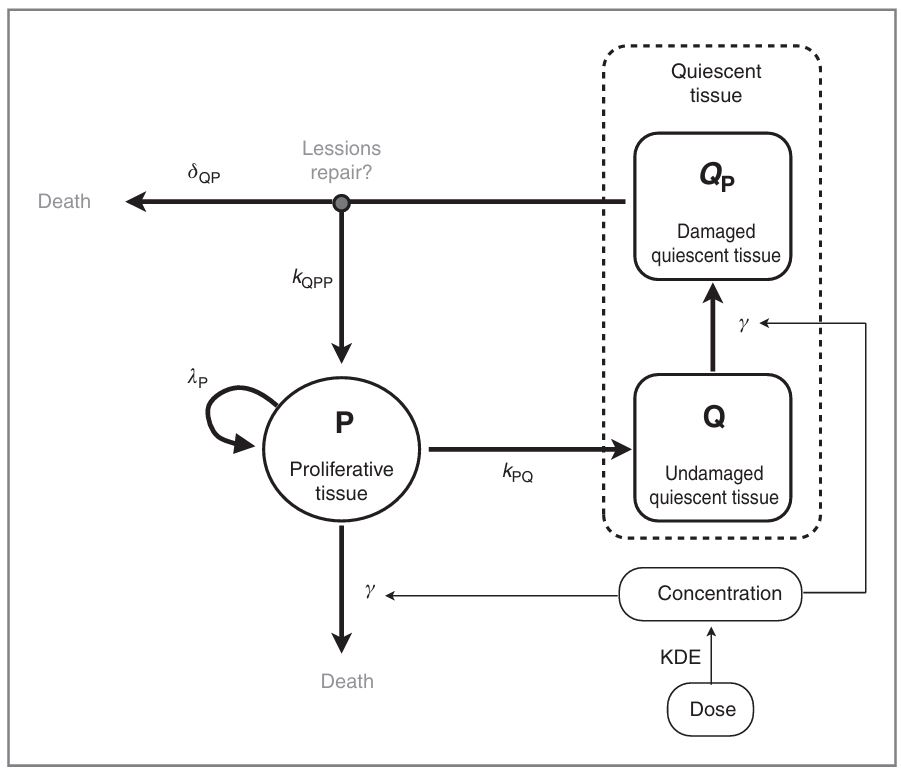
\includegraphics[width=\linewidth]{Image/modele.JPG} 
        \caption{} \label{fig:model}
    \end{subfigure}
    \hfill
    \begin{subfigure}[t]{0.45\textwidth}
        \centering
        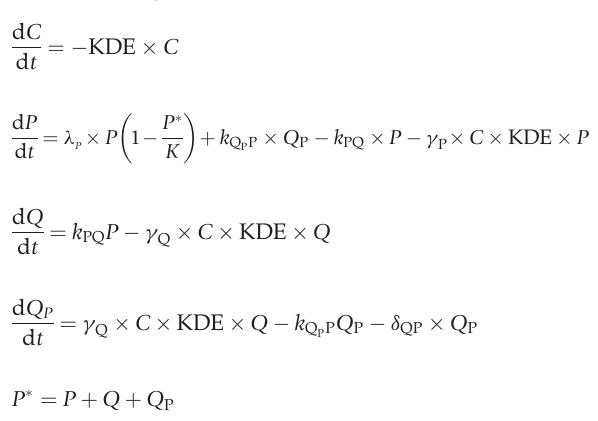
\includegraphics[width=\linewidth]{Image/eq.JPG} 
        \caption{} \label{fig:teq}
    \end{subfigure}

    \vspace{1cm}
    \begin{subfigure}[t]{\textwidth}
    \centering
        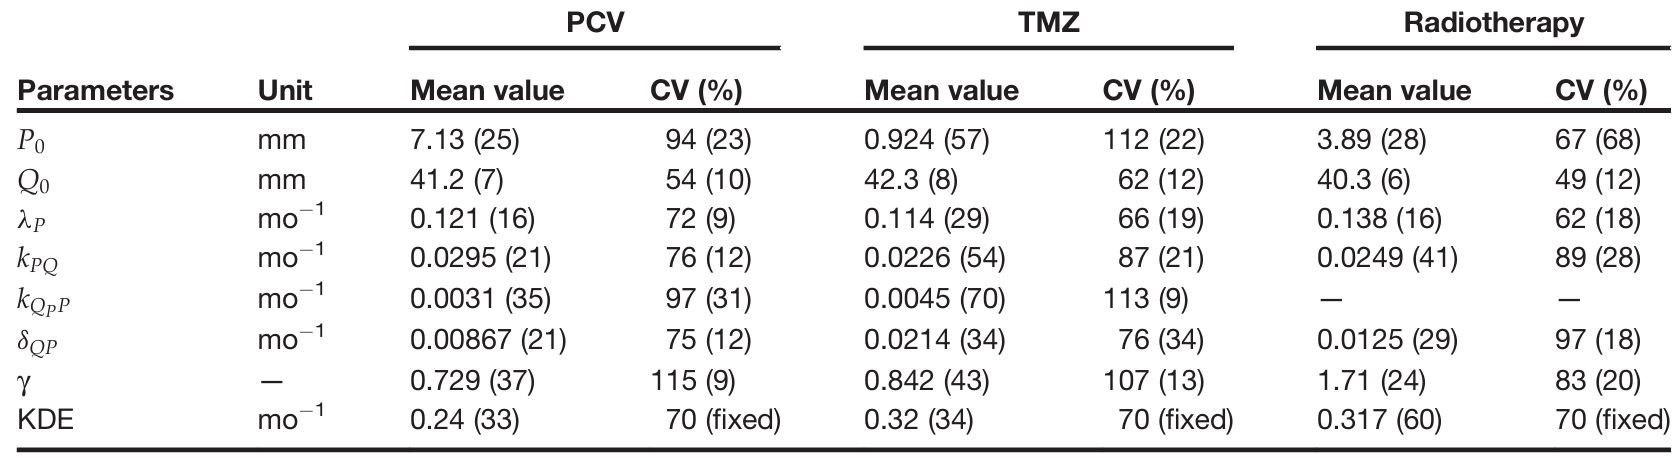
\includegraphics[width=\linewidth]{Image/tableau.JPG} 
        \caption{} \label{fig:tableau}
    \end{subfigure}
    
    \caption{\textbf{Présentation du modèle \cite{} (a).} Modèle à 3 compartiments $P$ (tissu prolifératif), $Q$ (tissu quiescent), $Q_{p}$ (tissu quiescent endommagé). Sous l'effet du traitement de concentration C (normalisée) qui va endommagé l'ADN des cellules, P peut être endommagé et mourir selon efficacité $\gamma$ et Q peut devenir $Q_p$ selon efficacité $\gamma$. $Q_{p}$ mourrir selon $\delta$ ou redevenir prolifératif. Les coefficients $k$ désigne la proprtion de tissu qui transitionne vers un autre état.  \textbf{(b).} Mise en équation du modèle proposé. \textbf{(c).} Estimation des paramètres d'après fitting de données de patients ayant subi les différents traitements au modèle. CV désigne le coefficient de variation qui caractérise la variabilité interindividuelle. L'erreur sur les estimations est donnée par les nombres entre parenthèses en pourcentage. Pour plus de précisions se référer à l'article référence\cite{}}
\end{figure}

\subsubsection{Explication du modèle}
Les équation différentielles sont résolues numériquement entre chaque évenement (début de simulation, injections, et fin de simulation) séquentiellement. Après chaque interval, la concentration d'agent chimique peut être ajustée, et le système ainsi modifié sert de point de départ pour l'interval suivant. Les temps pour lesquels les valeurs sont calculées sont répartis uniformément dans chaque interval, avec temps de debut et de fin inclus, mais ne le sont pas forcément entre chaque interval. Ceci a des impact pour la contruction de la fonction de calcul de score que nous expliquerons dans la section dédiée.
\subsubsection{Paramétrisation}
Dans l'article de référence, des données de patients ayant été traité par différentes thérapies: Chimiothérapies PCV, Chimiothérapies TMZ et radiothérapies; ont été utilisées pour paramétriser le modèle. Pour chacune de ces cohortes ils ont estimé des paramètres moyens et quantifier la variabilité interindividuelle par le coefficient de variation (CV) \ref{fig:tableau}.  On constate que pour les différents traitements, le DT évolue différemment \ref{fig:evol_moy}. $\lambda_{p}$ (coefficient de croissance du tissu), $P_{0}$ (tissu prolifératif à l'instant 0) et $Q_{0}$ (tissu quiescent à l'instant 0) sont des paramètres associés à la tumeur.  Ces paramètres peuvent être estimées sur les patients avant le début du traitement. On estime souvent P égal à 10\% du DT et on peut mesurer $\lambda_{p}$ sur la croissance de la tumeur pendant le pré-traitement. Une estimation individuelle du modèle permet de prédire avec plus de précision l'évolution du DT de la tumeur avec le modèle. En effet, ces paramètres notamment $\lambda_{p}$ varient beaucoup entre individus\ref{fig:tableau}. Or, comme on le constate des faibles variations de ces paramètres sont suffisantes pour modifier significativement  l'évolution du DT \ref{fig:rand_traj}. On fait varier le $DT_{0}$ entre 30 et 85mm et on définit $P_{0}$ comme 10\% (proportion observée cliniquement) du DT et on fait varier $\lambda_{p}$ selon sa distribution donnée pour le traitement PCV \ref{fig:tableau}. On choisit également les autres paramètres comme paramètres moyens de PCV. On observe des trajectoires différentes.  On  souhaite comprendre le rôle de ces différents paramètres sur l'évolution du DT. De même, les caractéristiques du traitement, $\gamma$, $C$ vont probablement influer sur l'évolution de la tumeur. On va donc explorer l'espace des paramètres pour évaluer l'influence de ces différents paramètres.  
\begin{figure}
    \centering
    \begin{subfigure}[t]{0.45\textwidth}
        \centering
        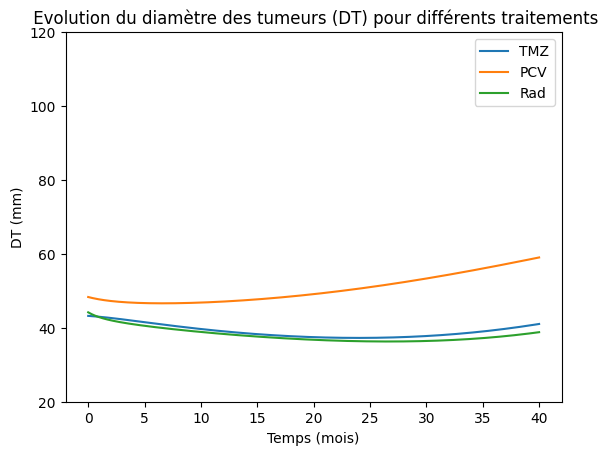
\includegraphics[width=\linewidth]{Image/evolution_TD_param_moy.png} 
        \caption{} \label{fig:evol_moy}
    \end{subfigure}
    \hfill
    \begin{subfigure}[t]{0.45\textwidth}
        \centering
        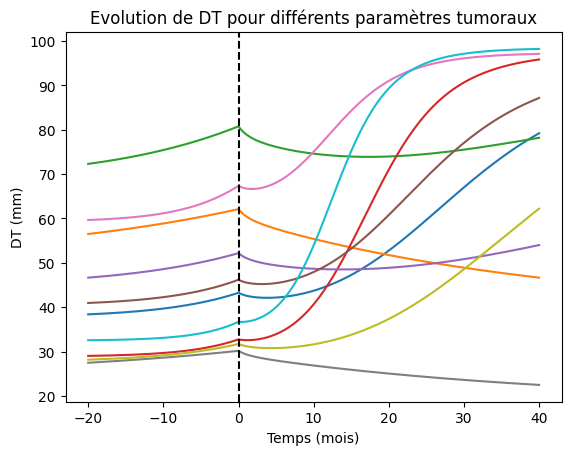
\includegraphics[width=\linewidth]{Image/ex_traj.png} 
        \caption{} \label{fig:rand_traj}
    \end{subfigure}

    \caption{\textbf{(a).} Evolution du diamètre d'une tumeur (DT) pour les paramètres de populations moyens des trois traitements chimiothérapie PCV, TMZ ou radiothérapie \cite{}. \textbf{(b).} Evolution du DT pour les paramètres moyens PCV sauf $\lambda_{p}$, $P_{0}$, $Q_{0}$ choisi aléatoirement selon les distributions les valeurs moyennes et coefficient de variation indiqué dans \ref{fig:tableau} Le traitement est injecté à t=0. }
\end{figure}

\subsection{Exploration de l'espace des paramètres}
On constate que des variations des paramètres tumoraux modifient significativement l'évolution du DT \ref{fig:rand_traj}.  On regarde l'influence de $\lambda_{p}$ et  la proportion de $\frac{P_{0}}{Q_{0}}$
sur le DT \ref{fig:heatmap}. On fait varier $P_{0}$ entre 3 et 15\% du DT qu'on fixe à 50mm, et $\lambda_{p}$ varie entre 0 et 0.4 qui représente les variations interindividuelles tous traitements confondus. On constate que $\lambda_{p}$ est déterminant pour le DT moyen sur 40 mois pour les trois traitements tandis que $\frac{P_{0}}{Q_{0}}$ n'a qu'une influence réduite. Mais ces deux paramètres ont des effets sur la proportion des différentes populations (figures non présentées). Toutefois, l'objectif des traitements est la diminution de la taille de la tumeur, et donc des trois types de tissu. Il semble qu'estimer $\lambda_{p}$ pour chaque patient est essentiel pour prédire le DT et paramétriser le modèle. Les paramètres du traitement,  $\gamma$ et C, sont également déterminant pour diminuer la taille de la tumeur. Augmenter la dose injectée $C_{0}$ permet réduire le DT moyen sur 40 mois. Toutefois, on constate qu'à partir d'une certaine concentration, le DT ne réduit plus \ref{fig:effet_C}. Toutefois, ici on ne considère pas la toxicité du traitement.  Or, ces traitements engendrent des dommages à l'ADN ce à haute dose est nocif pour les patients. Il faut ainsi évaluer la balance bénéfice risque. De même, augmenter $\gamma$, qui caractérise l'éfficacité des traitements pour créer des dommages ADN, diminue le DT moyen. Mais là encore on ne caratérise pas la nocivité pour les patients. Par ailleurs, on considère ici que $\gamma$ est constant. Or, on suppose qu' au cours du temps, les cellules traitées vont développer de la résistance. Le phénomène de résistance des cellules quiescentes est essentiel dans la ressurgence des cancers. Mais, si on considère des temps courts ( environ 40 mois), cette hypothèse est cohérente. 
\begin{figure}
    
    \begin{subfigure}[t]{\textwidth}
    \centering
        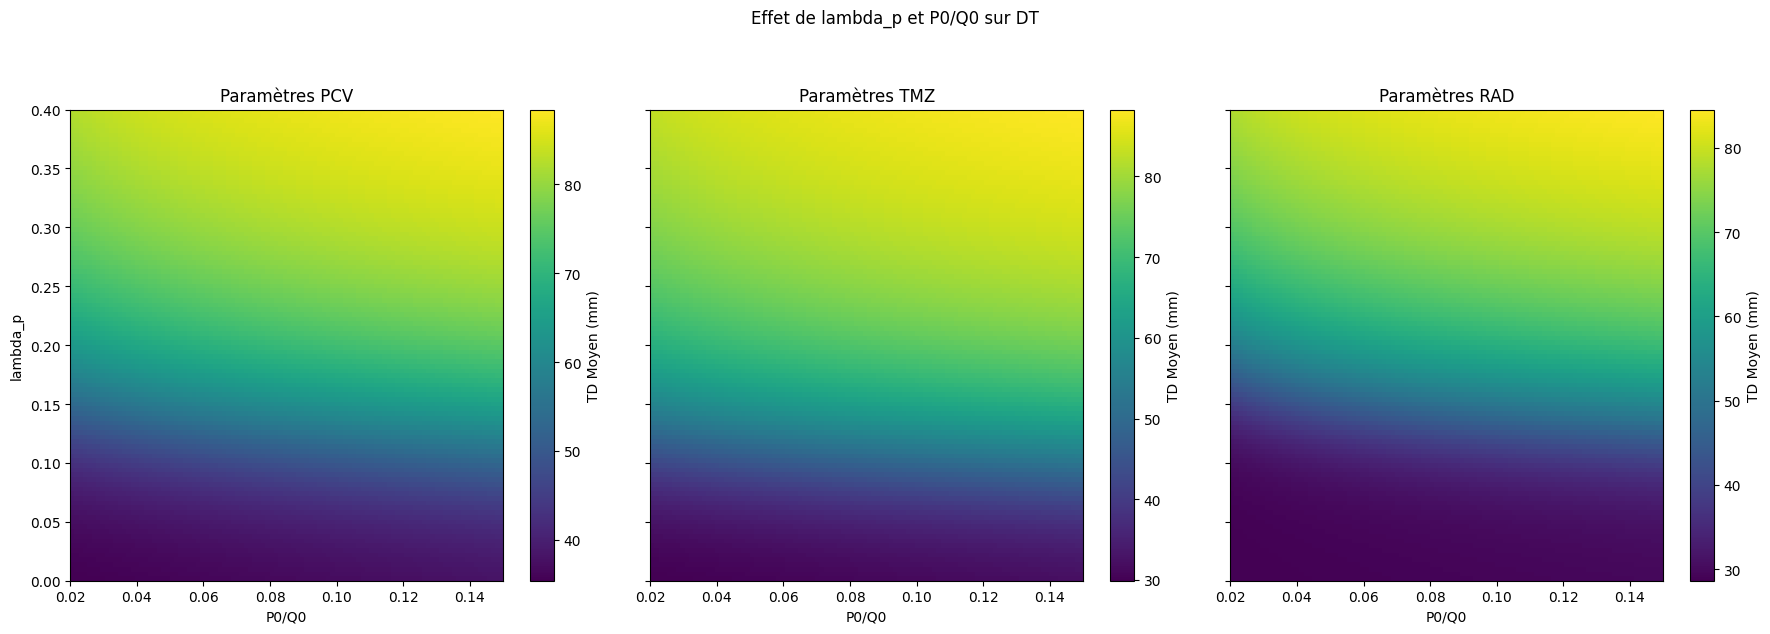
\includegraphics[width=\linewidth]{Image/heatmap_lambdap_p0Q0.png} 
        \caption{} \label{fig:heatmap}
    \end{subfigure}
    \vspace{1cm}
    \centering
    \begin{subfigure}[t]{0.45\textwidth}
        \centering
        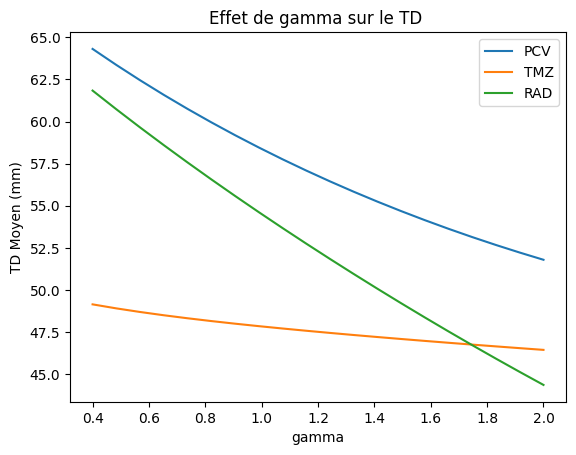
\includegraphics[width=\linewidth]{Image/effet_gamma.png} 
        \caption{} \label{fig:effet_gamma}
    \end{subfigure}
    \hfill
    \begin{subfigure}[t]{0.45\textwidth}
        \centering
        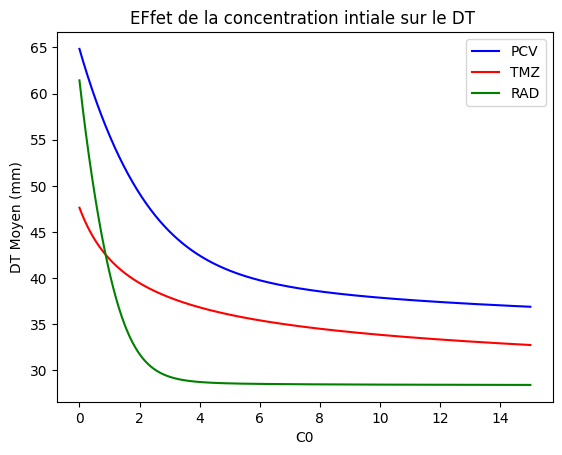
\includegraphics[width=\linewidth]{Image/effet_C.png} 
        \caption{} \label{fig:effet_C}
    \end{subfigure}

    \caption{\textbf{(a).} Effet de $\lambda_{p}$ et $\frac{P_{0}}{Q_{0}}$ sur le DT moyen, jaune indique un DT grand et bleu faible. \textbf{(b).} Effet de $\gamma$ sur le DT, les autres paramètres sont choisis selon les valeurs moyennes des traitements. \textbf{(c).} Effet de $C$ sur le DT, les autres paramètres sont choisis selon les valeurs moyennes des traitements.}

\end{figure}
Il semble donc essentielle d'estimer les paramètres individuelles des tumeurs et des traitements pour informer le modèle et prédire avec précision l'évolution du DT. 
Pour l'instant, on a considéré que les traitements sont injectés en une seule fois à t=0.  Mais est-ce qu'injecter la même dose de traitement en plusieurs fois ou à des proportions différentes de $P_{0}$, $Q_{0}$ pourrait diminuer le DT sans accroître excessivement la toxicité ? 
\section{Optimisation du moment et de la fréquence d'injection}
On cherche à établir le meilleur moment pour injecter une dose de traitement. Pour ce faire, on choisit un score S à minimiser. Ce score est l'intégrale du diamètre de la tumeur sur la durée de la simulation. L'objectif du traitement est de réduire la taille de la tumeur sur un temps long et non seulement de considérer le DT à un t doné car alors, les injections seraient faites au temps peu avant t. Le score choisit ainsi de la durée de la simulation
Comme expliqué précédement, les points de temps pour lesquels les différentes populations sont estimées ne sont pas répartis uniformément sur la durée de la simulation, et certains sont répétés. En effet, les valeurs de fin d'un interval (avant injection) et de debut de l'interval suivant (après injection) sont tous les deux dans les données, au même temps. Ainsi, afin de limiter l'opportunité de la fonction d'optimisation d'exploiter le systeme de sampling, par exemple en choisisant des temps d'injections permettant de surreprésenter la période de temps pendant laquelle la tumeur est petite pour diminuer artificiellement le score, nous utilisons une intégration par méthode des trapèzes au lieu de prendre la moyenne des tailles. Cela n'élimine cependant pas la sous-estimation sur les parties convexes du \ac{DT}.

\subsection{Optimisation pour une unique injection}
On cherche d'abord à déterminer si injecter le traitement à $ t > 0$  réduit S.  On observe le DT moyen pour des simulations de durée variable \ref{fig:duree_simu}. Si le temps de simulation est inférieure à 60 mois, pour les paramètres moyens des différents traitements, on voit qu'il est préférable de réaliser l'injection à t=0.  Pour les trois traiments à partir d'une certaine durée de simulation, le moment d'injection (MI) augmente linéairement en fonction de la durée de simulation. Mais on a considéré ici les paramètres moyens uniquement, or on a constaté précedemment que $\lambda_{p}$ avait un effet significatif sur l'évolution des tumeurs. On regarde donc si pour des simulations courtes (60 mois), des $\lambda_{p}$ différents il est également optimal de choisir $MI = 0$ \ref{fig:effet_lambda_moment}. On voit que pour PCV notamment, si la tumeur crôit plus vite que la moyenne, il est préférable de retarder l'injection. Mais il semble tout de même que $MI = 0$ est optimal.
\begin{figure}

    \centering
    \begin{subfigure}[t]{\textwidth}
        \centering
        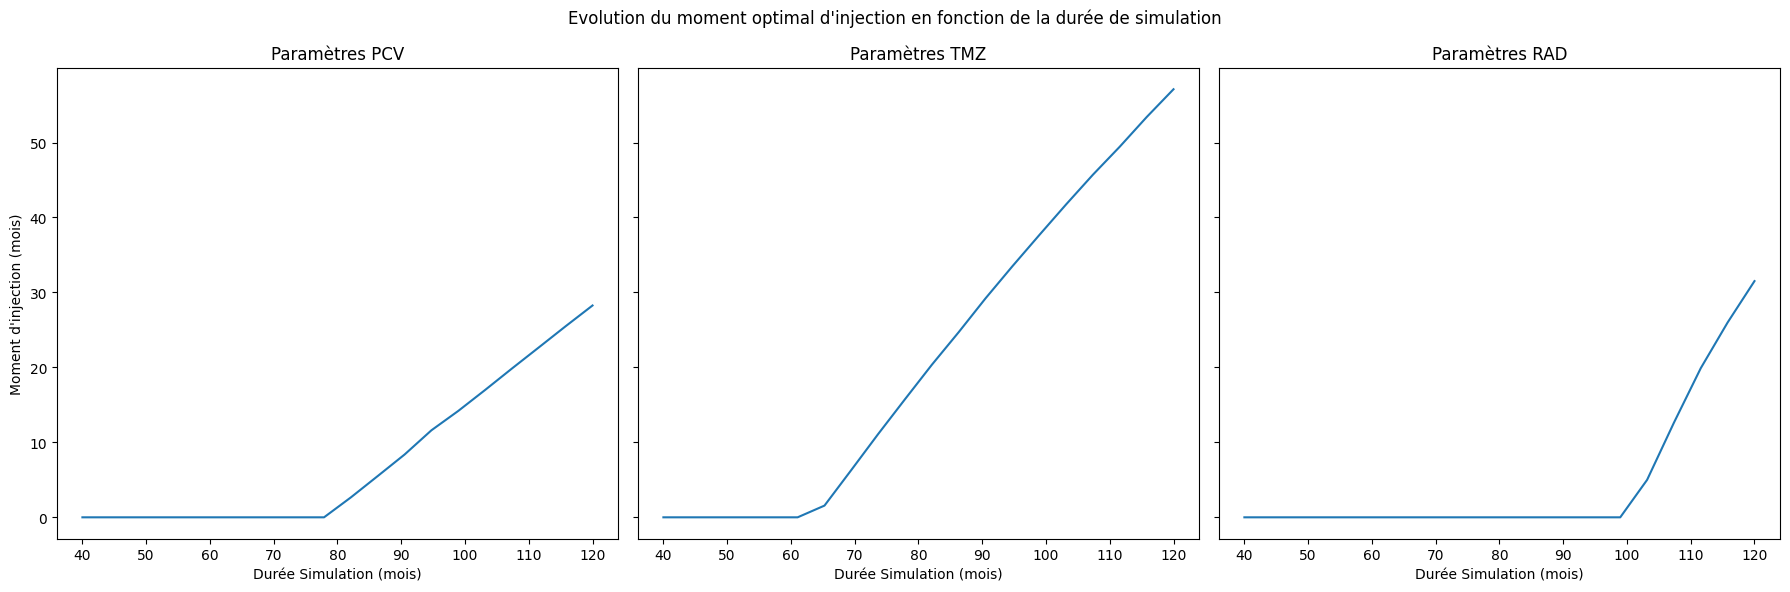
\includegraphics[width=\textwidth]{Image/duree_simu.png} 
        \caption{} \label{fig:duree_simu}
    \end{subfigure}

    \vspace{0.5cm}

    \begin{subfigure}[t]{\textwidth}
        \centering
        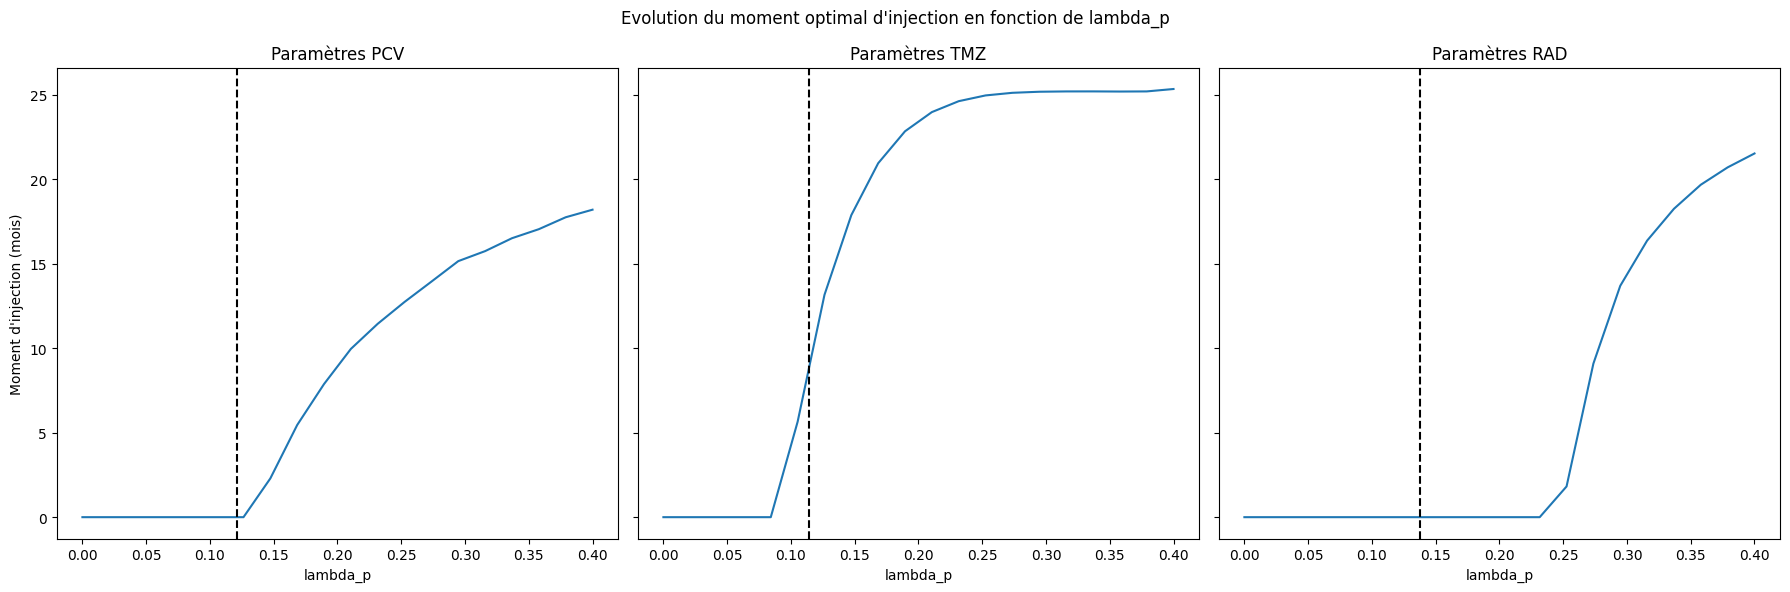
\includegraphics[width=\textwidth]{Image/effet_lambda_moment.png}
        \caption{} \label{fig:effet_lambda_moment}
    \end{subfigure}

    \caption{\textbf{(a).} DT moyen pour des simulations de durée entre 20 et 120 mois pour les paramètres moyens des différents traitements. \textbf{(b).} Effet de $\lambda_{p}$ sur le DT pour une durée de simulation de 60 mois.}
\end{figure}
\subsubsection{Moment d'injection optimal en fonction de la quantité injectée}
%Paul

\subsection[Injections répétées]{Minisation de la taille moyenne de la tumeur par injections répétées}
%Paul
\subsubsection{Principes généraux}
L'objectif est de savoir si en réalisant $n_{inj}$ injections, le \ac{DTM} peut être réduit. 
Pour trouver les minima globaux, notre première méthode était de trouver une estimation grossière en explorant de l'ensemble des valeurs des \acp{MI} possibles par une grille à $n_{inj}$ dimensions, avec $N=20$ points par dimensions, par \texttt{scipy.optimise.brute}. Cette estimation était ensuite  minimisée localement par \texttt{scipy.optimize.minimise} avec la methode L-BGCF-B\cite{}.\\
Le premier problème était que la complexité de la première étape de cette méthode $O({N}^{n_{inj}})$ rendait cette méthode peu pratique pour des calculs à haute dimention ($n_{inj}\geq4$). Cependant, nous avions remarqué que la distribution des \acp{MI} optimaux proposée ressemblait à un espacement régulier des injections. Ainsi, nous avons choisi de déteminer le protocole optimal en deux étapes. Premièrement, nous cherchions un protocole avec un interval de temps régulier $\delta_{t}$ entre les injections, à partir temps de première injection $T_{i}$. Ces deux paramètres étaient trouvées par exploration grossière en grille, suivi d'une minimisation locale. Les \acp{MI} ainsi optenus servent de point de départ pour la recherche du protocol optimal sans contrainte d'un interval régulier.\\
En comparant ces deux résultats, nous pouvons aussi évaluer le coût d'imposer des injections espacées d'un temps régulier.

\subsubsection[Injections multiples 120 mois]{Evolution de \acf{DTM} sur 120 mois en fonction du nombre d'injections}
\subsubsection{}

\section{Conclusion}
Ce modèle peut s'avérer utile pour prédire l'évolution de la taille de la tumeur si les propriétés de la tumeur on pu être établies avant le traitement \cite{}. Il apparaît donc comme un potentiel outil de thérapie personalisée pour optimiser chez chaque patient le moment et les fréquences d'injection.  De plus, d'utres cancer tel que le cancer du sein ou du poumon, présentent des tissus P, Q et $Q_{p}$. Il serait intéressant de fitter ce modèle sur des données de patients pour tester sa validité. Mais le modèle tel qu'ici présenté a également de multiples limitations. 
\subsection{Limites et Perspectives}
Tout d'abord, les données de patients à disposition n'ont permis uniquement d'observer les réponses au traitement des patients sur 40 à 60 mois.  Le modèle paraît valide pour des temps courts mais sa validité reste à tester sur des temps plus longs. En effet, sur des temps court on peut supposer que le développement de résistance aux traitements par les cellules tumorales est négligeable. Mais sur des temps longs, ce phénomène est essentielles dans la ressurgence de cancer plus aggressif. Il serait souhaitable de modifier le modèle pour inclure ce phénomène. \\
Par ailleurs, ici on a considéré des patients suivant un unique traitement, or souvent les chimiothérapies sont prescrites après une chirurgie et radiothérapie. Il serait intéressant de modéliser les réponses aux traitements combiner afin de proposer une stratégie thérapeutique personnalisé.\\
Des nouveaux traitements depuis la parution de l'article qui n'utilise pas les même mécanismes ... 
\end{document}